%%%%%%%%%%%%%%%%%%%%%%%%%%%%%%%%%%%%%%%%%%%%%%%%%%%%%%%%%%%%%%%%%%%%%%%%%%%%%%%%%%%%%%%%%%%%%%%%%%%
%%%%%%%%%%%%%%%%%%%%%%%%%%%%%%%%%%%%%%%%%%%%%%%%%%%%%%%%%%%%%%%%%%%%%%%%%%%%%%%%%%%%%%%%%%%%%%%%%%%
%%%%%%%%%%%%%%%%%%%%%%%%%%%%%%%%%%%%%%%%%%%%%%%%%%%%%%%%%%%%%%%%%%%%%%%%%%%%%%%%%%%%%%%%%%%%%%%%%%%

\chapter{Espectro de potencias}

Existe una larga tradición para entender y modelar las señales electrofisiológicas en términos de 
\textit{ondas y frecuencias}, ya que fundamentalmente son fenómenos eléctricos \cite{Kaiser00}.
%
%Se aborda el enfoque usual del espectro de potencias: se asocia la energía de una señal con su 
%dispersión (varianza) y se estudia cómo se distribuye en la base de Fourier.
%%
%En el entendido de que el espectro de potencias puede variar en el tiempo, la estacionariedad
%es equivalente a que el tal cambio no ocurra.
%
En este capítulo se expone el enfoque \textit{usual} en cuanto a modelar las señales electrofisiológicas como procesos estocásticos a los cuales se puede definir un \textit{espectro de potencias}.
%
El espectro de potencias es entendido como una generalización para el módulo de la transformada de Fourier; conserva algunas de sus propiedades, como el ser una norma inducida por un producto interno, así como la interpretación asociada como distribución de \textit{energía}.

%La sección \ref{sec:fourier1} trata específicamente sobre la transformada de Fourier y algunas de sus propiedades, así como algunas de sus generalizaciones para varios espacios importantes en el contexto de series fisiológicas.
%
En la sección \ref{sec:fde} se define el espectro de potencias para procesos estocásticos débilmente estacionarios y se establecen condiciones de existencia; la discusión sobre unicidad se ubica en la sección \ref{sec:representacion}, donde se define una forma de representar al proceso en términos de su espectro.
%
Finalmente, la sección \ref{sec:estimadores} trata sobre la estimación del espectro de un proceso a partir de una realización del mismo; se aborda el enfoque de obtener una versión \textit{suavizada} del espectro en aras de que los estimadores sean consistentes.

Un hecho que conviene reiterar es que todos los temas son expuestos dos veces: para procesos estocásticos a tiempo continuo y para aquellos a tiempo discreto; 
%
Cabe mencionar que en este capítulo se trata únicamente el caso de procesos estocásticos \textit{débilmente estacionarios}, mientras que en el siguiente se explora una familia más general de procesos estocásticos.
%
Dentro del contexto global del presente trabajo, el capítulo entero pudiera etiquetarse como el estudio de un caso particular salvo por simplicidad expositiva.

%%%%%%%%%%%%%%%%%%%%%%%%%%%%%%%%%%%%%%%%%%%%%%%%%%%%%%%%%%%%%%%%%%%%%%%%%%%%%%%%%%%%%%%%%%%%%%%%%%%
%%%%%%%%%%%%%%%%%%%%%%%%%%%%%%%%%%%%%%%%%%%%%%%%%%%%%%%%%%%%%%%%%%%%%%%%%%%%%%%%%%%%%%%%%%%%%%%%%%%



\section{Función de densidad espectral}
\label{sec:fde}

La forma más \textit{natural} de definir un espectro de potencias para un proceso estacionario es a través de la transformada de Fourier de sus realizaciones. 
%
Tal enfoque no funciona en general, pues no se puede garantizar que las realizaciones arbitrarias admitan una transformada de Fourier (ni aún de Fourier-Stieltjes).
%
Se define entonces el espectro en base a un límite de subcolecciones de la realización, de modo que éstas sí admitan una transformada de Fourier.

\begin{definicion}[Función de densidad espectral, tiempo continuo]
Sea \xt un proceso estacionario a tiempo continuo. Se define su {función de densidad 
espectral} como
\begin{equation}
h(\omega) = \frac{1}{2 \pi} \lim_{T\rightarrow \infty} \E{ \frac{1}{2T} 
\abso{ \int_{-T}^{T} X(t) e^{-i \omega t} dt}^{2} }
\label{txt_FDE_cont}
\end{equation}
\end{definicion}

%De la defunción se deduce que la función de densidad espectral (FDE) siempre es una función
%no-negativa

[? ejemplos: ruido rosa esta bien definido, proceso oscilatorio no esta definido, ruido blanco no esta definido]

\begin{definicion}[Función de densidad espectral, tiempo discreto]
Sea $\{X(t)\}_{\nicefrac{t}{\Delta_t}\in \Z}$ un proceso estacionario a tiempo discreto. Se 
define su {función de densidad espectral} como
\begin{equation}
h(\omega) = \frac{1}{2 \pi} \lim_{N\rightarrow \infty} \E{ \frac{1}{2N} 
\abso{ \sum_{n=-N}^{N} X(n \Delta_t) e^{-i \omega n \Delta_t}}^{2} }
\label{txt_FDE_disc}
\end{equation}
\end{definicion}

%%%%%%%%%%%%%%%%%%%%%%%%%%%%%%%%%%%%%%%%%%%%%%%%%%%%%%%%%%%%%%%%%%%%%%%%%%%%%%%%%%%%%%%%%%%%%%%%%%%
%%%%%%%%%%%%%%%%%%%%%%%%%%%%%%%%%%%%%%%%%%%%%%%%%%%%%%%%%%%%%%%%%%%%%%%%%%%%%%%%%%%%%%%%%%%%%%%%%%%

\section{Representación espectral}
\label{sec:representacion}

\begin{teorema}
Sea \xt un proceso continuo de media cero, débilmente estacionario, y que admite una función de densidad espectral $h$, sea $R$ su función de autocovarianza. Entonces
\begin{equation}
h(\omega) = \frac{1}{2\pi} \intR e^{i \omega \tau} R(\tau) d\tau
\end{equation}
\label{teo:corr_four}
\end{teorema}
\begin{proof}
Usando que $h = \lim_{T\rightarrow\infty} G_T$, nótese que
\begin{align*}
\abso{G_T(\omega)}^{2} &= 
\intR e^{i \omega t} \left[ \left(\frac{1}{\sqrt{2\pi}} \right)^{2} \intR X_T(u) X_T(u-\tau) du \right] d\tau \\
&=
\frac{1}{2\pi} \intR e^{i \omega t} \left[ \intR X_T(u) X_T(u-\tau) du \right] d\tau \\
\end{align*}
Esta integral puede verse como la transformada de Fourier de la función de autocorrelación de la serie truncada, $\widehat{R}_T$
\begin{align*}
\widehat{R}_T (\tau) &= \frac{1}{2T} \intR X_T(u) X_T(u-\tau) du \\
&= \begin{cases}
\frac{1}{2T} \int_{-T+\abso{\tau}}^{T} X(u) X(u-\abso{\tau}) du &, \abso{\tau} \leq T \\
0 &, \text{otro caso}
\end{cases}
\end{align*}
Así entonces
\begin{align*}
h(\omega) &=
\lim_{T\rightarrow \infty} \E{\frac{1}{2T} \abso{G_T(\omega)}^{2}} \\
&=
\lim_{T\rightarrow \infty}
\E{\frac{2T}{2\pi} \intR e^{i \omega t} \widehat{R}_T(\tau) d\tau }\\
&=
\frac{1}{2\pi}
\lim_{T\rightarrow \infty}
2T \intR e^{i \omega t} \E{\widehat{R}_T(\tau)} d\tau\\
\end{align*}
Para esto, si $\abso{\tau} \leq 2T$
\begin{align*}
\E{\widehat{R}_T(\tau)} &=
\E{\frac{1}{2T} \intR X_T(u) X_T(u-\tau) du} \\
&=
\E{ \frac{1}{2T} \int_{-T+\abso{\tau}}^{T} X(u) X(u-\tau) du } \\
&=
\frac{1}{2T} \int_{-T+\abso{\tau}}^{T} \E{X(u) X(u-\tau)} du \\
&=
\frac{1}{2T} \int_{-T+\abso{\tau}}^{T} R(\tau) du \\
&=
\frac{1}{2T} \left( 1 - \frac{\abso{\tau}}{2T} \right) R(\tau)
\end{align*}
pero si $\abso{\tau}>2T$ entonces $\widehat{R}_T = 0$. Luego entonces
\begin{align*}
h(\omega) &=
\frac{1}{2\pi} \lim_{T\rightarrow \infty}
\int_{-T}^{T} e^{i \omega t} \left( 1 - \frac{\abso{\tau}}{2T} \right) R(\tau) d\tau\\
&=
\frac{1}{2\pi} \lim_{T\rightarrow \infty}
\intR e^{i \omega t} g_T(t) R(\tau) d\tau
\end{align*}
con
\begin{equation}
g_T = \begin{cases}
1 - \nicefrac{\abso{\tau}}{2T} &, \abso{\tau} \leq 2T \\
0 &, \text{otro caso}
\end{cases}
\end{equation}

Para establecer el límite anterior nótese que para cualesquiera $\tau, T$ se cumple que $0\leq g_\tau \leq 1$, entonces
\begin{align*}
\intR e^{i \omega t} g_T(t) R(\tau) d\tau
&\leq
\abso{\intR e^{i \omega t} g_T(t) R(\tau) d\tau } \\
&\leq
\intR \abso{g_T(\tau)} \abso{ R(\tau)} d\tau \\
&\leq
\intR \abso{ R(\tau)} d\tau 
\end{align*}

%Suponiendo que $\intR \abso{ R(\tau)} d\tau < \infty$. 
Para cada $\omega$, el módulo de $\int_{-T}^{T} e^{i \omega t} g_\tau(t) R(\tau) d\tau$ es monótonamente creciente y acotado, luego entonces, por el teorema de convergencia dominada de Lebesgue, se tiene que
\begin{align*}
h(\omega) &=
\frac{1}{2\pi} \lim_{T\rightarrow \infty}
\intR e^{i \omega t} g_T(t) R(\tau) d\tau\\
&=
\frac{1}{2\pi} 
\intR e^{i \omega t} \left[ \lim_{T\rightarrow \infty} g_T(t) \right] R(\tau) d\tau\\
&=
\frac{1}{2\pi} 
\intR e^{i \omega t} R(\tau) d\tau\\
\end{align*}
\end{proof}

Es posible definir una \textbf{función de espectro integrado}, $H$, como
\begin{equation}
H(\omega_2) - H(\omega_1) = \frac{1}{2 \pi} \int_{\omega_1}^{\omega_2} h(\omega) d\omega =
\frac{1}{2\pi} \intR \frac{e^{i \omega_2 \tau}-e^{i \omega_1 \tau}}{i \tau} R(\tau) d\tau
\end{equation}

Usando que $h$ es una función simétrica tal que $\intR h(\omega) d\omega = \sigma_X^{2}$, entonces puede escribirse
\begin{equation}
H(\omega) = \frac{\sigma_X^{2}}{2} + \frac{1}{2 \pi} \intR \frac{e^{i \omega_1 \tau}-1}{i \tau} R(\tau) d\tau = \frac{\sigma_X^{2}}{2} + \frac{1}{2 \pi} \intR \frac{\SEN{\omega \tau}}{\tau} R(\tau) d\tau
\end{equation}

Conviene remarcar que el teorema \ref{teo:corr_four} sólo aplica si el proceso admite una función de densidad espectral, y en consecuencia no es claro si el espectro integrado queda bien definido para procesos que no admiten una densidad espectral. 
%
Por ejemplo, considérese el proceso $P$ definido como 
%$$ P(t) = \int_{t-\nicefrac{1}{2}}^{t+\nicefrac{1}{2}} \overline{\varepsilon} $$

El siguiente teorema permite establecer condiciones generales para las cuales se puede definir un espectro de potencias para un proceso estacionario.

\begin{teorema}[Wiener-Khintchine]
Una condición suficiente y necesaria para que $\rho$ sea una función de autocorrelación de 
algún proceso estocástico a tiempo continuo \xt débilmente estacionario y 
estocásticamente continuo, es que exista una función $F$ que tenga las siguientes propiedades
\begin{itemize}
\item Monótonamente creciente
\item $F(-\infty) = 0$
\item $F(+\infty) = 1$
\end{itemize}
y tal que para todo $\tau \in \R$ se cumple que
\begin{equation*}
\rho(\tau) = \intR e^{i \omega \tau} dF(\omega)
\end{equation*}
Como notación, el factor $dF$ será referido como la \textit{función de espectro integrado normalizado} para el proceso.
\label{t_wienerkhinchin}
\end{teorema}

Una vez definido y probada la existencia de la función de espectro integrado normalizado $dF$, se define la \textbf{función de espectro integrado} $dH$ (sin el adjetivo \textit{normalizado}) como
$dH := \sigma_X^{2} dF$.

%%%%%%%%%%%%%%%%%%%%%%%%%%%%%%%%%%%%%%%%%%%%%%%%%%%%%%%%%%%%%%%%%%%%%%%%%%%%

Una vez establecidas las condiciones de existencia para el espectro de potencias de un proceso débilmente estacionario, una pregunta muy natural es sobre la unicidad.
%
Cuando se discutió la transformada de Fourier para funciones en $L^{2}$, se dejó en claro que es un operador invertible salvo por su núcleo (definición ?).

Se mostró que la transformada de Fourier puede ser parameterizada en módulo y argumento, siendo el primero es equivalente (salvo una función invertible) al espectro.
%
El espectro de un proceso estacionario fue definido como
\begin{align*}
h(\omega) &= \lim_{T\rightarrow\infty} \E{\abso{ G_T(\omega)}^{2}} \\
G_T(\omega) &= \int_{-T}^{T} e_{i \omega t} X(t) dt
\end{align*}
la componente $G_T$ cumple intuitivamente el papel de la transformada de Fourier, pero es omitida para demostrar más fácilmente la existencia del espectro $h$. Contemplando la parametrización de la transformada de Fourier, ¿puede definirse algo equivalente al argumento para un proceso estacionario?
%
%Un enfoque propuesto por Winer [citar, 1930, capitulo 1] es
[? mejorar redacción]

\begin{teorema}
Sea \xt un proceso a tiempo continuo, débilmente estacionario, de media 0 y estocásticamente continuo en el sentido de media cuadrática. Existe un proceso ortogonal $\{Z(\omega)\}$ tal que, para todo tiempo $\omega$ admisible, se puede escribir
\begin{equation*}
X(t) = \intR e^{i t \omega} dZ(\omega)
\end{equation*}
Donde el proceso $\{Z(t)\}$ tiene las siguientes propiedades para todo $\omega$
\begin{itemize}
\item $\E{dZ(\omega)} = 0$
%\item $\E{\abso{dZ(\omega)}^{2}} = dH(\omega)$
\item $\Cov{dZ(\omega),dZ(\lambda)} = dH(\omega) \delta(\omega, \lambda)$
\end{itemize}
Donde $dH(\omega)$ el espectro integrado de \xt
\label{rep_espectral}
\end{teorema}

%\begin{proof}
%Se considera a \xt, un proceso que satisface las condiciones del teorema, y a $\{x(t)\}_{t\in \mathcal{T}}$, una realización. Se define $x_T$, una extensión periódica de la restricción de longitud $T$ para $x$, como
%%\begin{equation}
%%x_T(t) = x\left( 2T \entero{\frac{t+T}{2T}} -T \right)
%%\end{equation}
%\begin{equation}
%x_T(t) = \begin{cases}
%x(t) &, \abso{t} \leq T \\
%x(t_*+2pT) &, p \text{ tal que } \abso{t_*}\leq T
%\end{cases}
%\end{equation}
%Como $x_T$ es periódica, con periodo $2T$, puede escribirse como
%\begin{align*}
%x_T(t) &= \sum_{n=-\infty}^{\infty} A_n e^{i \nicefrac{2\pi n t }{T}} \\
%A_n &= \frac{1}{2T} \int_{-T}^{T} x_T(t) e^{-i \nicefrac{2\pi n t }{T}}
%\end{align*}
%Se define entonces una función $G_T$, análoga a la usada al definir el espectro, como
%\begin{equation}
%G_T(\omega) = \int_{-T}^{T} \frac{1}{\sqrt{2 \pi}} x_T(t) e^{i \omega t} dt = \int_{-T}^{T}     \frac{1}{\sqrt{2 \pi}} x_T(t) e^{i \omega t} dt
%\end{equation}
%Luego entonces, puede escribirse
%\begin{equation}
%asdasd
%\end{equation}
%\end{proof}

\begin{proof}
Se mostró anteriormente que $\mathcal{R}$, el conjunto de variables aleatorias con media cero y varianza finita, tiene la estructura de espacio de Hilbert con el producto interno
\begin{equation}
\langle U , V \rangle := \Cov{U,V} = \E{U, \overline{V}}
\end{equation}
Ahora bien, un proceso débilmente estacionario \xt puede verse como una \textit{curva} en $\mathcal{R}$ indexada por $t \in \mathcal{T}$.
%
Por el teorema de Winer-Khintchine, existe un proceso ortogonal $dH$ tal que puede escribirse
\begin{equation}
\pint{X(t),X(s)} = R(t-s) = \intR e^{i \omega (t-s)} dH(\omega)
\end{equation} 
De manera más general, puede hablarse de una familia de funciones $\{ \phi_t \}_{t\in \mathcal{T}}$ (anteriormente se usó $\phi_t(\omega) = e^{i \omega t}$) y escribir
\begin{equation}
\pint{X(t),X(s)} = \intR \phi_t(\omega) \overline{\phi_s(\omega)} dH(\omega)
\end{equation} 
Usando la familia de funciones $\{ \phi_t \}_{t\in \mathcal{T}}$ puede construirse un segundo espacio de Hilbert, $\mathcal{H}_\phi$, como las combinaciones lineales de estas funciones.
A este segundo espacio se le define el producto interno
\begin{equation}
\pint{\phi_1,\phi_2}_H := \intR \phi_1(\omega) \overline{\phi_2(\omega)} dH(\omega)
\end{equation} 
Posteriormente se define un mapeo $M : \mathcal{H}_\phi \rightarrow \mathcal{R}$ como
\begin{equation}
M[\phi_t] := X(t)
\end{equation}
el cual se extiende linealmente para cualesquiera coeficientes $c_1, c_2, \cdots \in \R$ y tiempos admisibles $t_1, t_2, \cdots \in \mathcal{T}$
\begin{equation}
M\left[ \sum_i c_i \phi_{t_i} \right] = \sum_i c_i M\left[ \phi_{t_i} \right]
\end{equation}
Trivialmente, $M$ conserva productos internos; basta notar que
\begin{equation}
\pint{X(t),X(s)} = \intR \phi_1(\omega) \overline{\phi_2(\omega)} dH(\omega) = \pint{\phi_1,\phi_2}_H
\end{equation}
Ahora, para trabajar con las funciones $\phi$ conviene descomponerlas en una base más \textit{sencilla}, como límite de funciones simples. Para ello, se define una función indicadora
\begin{equation}
I(\omega; \omega_0, \omega_f) := \begin{cases}
1 &, \omega_0 \leq \omega < \omega_f \\
0 &, \text{otro caso}
\end{cases}
\end{equation}
Luego, sea $\{\omega_0, \omega_1, \cdots, \omega_N\}$ una partición del intervalo $[-n,n]$, con $n>>N$. Entonces, en virtud del teorema de convergencia dominada de Lebesgue
\begin{equation}
\phi_t(\omega) = \lim_{n\rightarrow\infty} \sum_{i=1}^{N} I(\omega; \omega_{i-1}, \omega_i) \left[  \inf_{\omega \in [\omega_{i-1},\omega_i]} \phi_t(\omega_{i})\right]
\label{asd}
\end{equation}
Usando tal representación para las funciones $\phi$'s, se define a $Z$ como
\begin{equation}
Z(\omega_f) - Z(\omega_0) = M\left[ I(\omega; \omega_f, \omega_0) \right]
\end{equation}
Luego entonces, aplicando $M$ a ambos lados de la expresión \ref{asd} se obtiene
\begin{align*}
M\left[ \phi_t(\omega) \right] &= M\left[ \lim_{n\rightarrow\infty} \sum_{i=1}^{N} I(\omega; \omega_{i-1}, \omega_i) \left[  \inf_{\omega \in [\omega_{i-1},\omega_i]} \phi_t(\omega_{i})\right] \right] \\
&= \lim_{n\rightarrow\infty} \sum_{i=1}^{N} M\left[I(\omega; \omega_{i-1}, \omega_i) \right] \left[  \inf_{\omega \in [\omega_{i-1},\omega_i]} \phi_t(\omega_{i})\right] \\
&= \lim_{n\rightarrow\infty} \sum_{i=1}^{N} \left( Z(\omega_i) - Z(\omega_{i-1})\right) \left[  \inf_{\omega \in [\omega_{i-1},\omega_i]} \phi_t(\omega_{i})\right] \\
&= \intR \phi_t(\omega) dZ(\omega)
\end{align*}
El resultado que se busca queda establecido porque $M[\phi_t] = X(t)$
\begin{equation}
X(t) = \intR \phi_t(\omega) dZ(\omega)
\end{equation}
\end{proof}



\subsection{Representación de procesos a tiempo discreto}

La existencia de espectros para procesos a tiempo discreto es dada por el teorema

\begin{teorema}[Wold]
Una condición suficiente y necesaria para que $\rho$ sea una función de autocorrelación de 
algún proceso estocástico a tiempo discreto \xt débilmente estacionario es que exista 
una función $F$ con las siguientes propiedades
\begin{itemize}
\item Monótonamente creciente
\item $F(-\pi) = 0$
\item $F(+\pi) = 1$
\end{itemize}
y tal que para todo $\tau \in \R$ se cumple que
\begin{equation*}
\rho(\tau) = \intPI e^{i \omega \tau} dF(\omega)
\end{equation*}
\label{t_wold}
\end{teorema}

\begin{proof}
Por simplicidad, supóngase que $\Delta_X=1$. A tiempo discreto, la función de autocovarianza adquiere la forma de una secuencia $\{R(\tau)\}_{\tau\in \Z}$. Se define una función $R_C$ que es igual a $R$ pero cuyo dominio es $\R$, de la forma
\begin{equation}
R_C(\tau) = \left( 1 - \tau + \entero{\tau} \right) R\left( \entero{\tau} \right) +
\left( s - \entero{\tau} \right) R\left( \entero{\tau} +1 \right)
\end{equation}
Se demuestra en Priestley 1963 [?] que existe un proceso estacionario cuya función de autovarianza es $R_C$, luego entonces por el teorema \ref{t_wienerkhinchin} existe una función de distribución $Q$ tal que 
\begin{equation}
R_C(\tau) = \intR e^{i \omega \tau} dQ(\omega)
\end{equation}
Dado que $R$ y $R_C$ son iguales cuando $\tau$ es entero, se puede considerar la siguiente manipulación con $\tau \in \Z$.
\begin{align*}
R(\tau) &= 
\intR e^{i \omega \tau} dQ(\omega) \\
&=
\sum_{s = -\infty}^{\infty} \int_{(2s-1)\pi}^{2s+1 \pi} e^{i \omega \tau} Q(\omega) \\
&=
\sum_{s = -\infty}^{\infty} \int_{-\pi}^{\pi} e^{i \left(\omega + 2\pi s \right) \tau} Q(\omega + 2 \pi s) \\
&=
\sum_{s = -\infty}^{\infty} \int_{-\pi}^{\pi} e^{i \omega \tau} Q(\omega + 2 \pi s) \\
&=
\int_{-\pi}^{\pi} e^{i \omega \tau} \left[ \sum_{s = -\infty}^{\infty} Q(\omega + 2 \pi s) \right] \\
\end{align*}
Finalmente se puede definir a $F$, la función de densidad descrita por el teorema, usando
\begin{equation}
dF(\omega) = \sum_{s = -\infty}^{\infty} Q(\omega + 2 \pi s)
\end{equation}
El que $F$ sea monótonamente se deduce de que $Q$ lo es. Como $dQ$ es simétrica, puede definirse convenientemente que $F(-\pi)=0$ y $F(\pi) = 1$ con base a que
\begin{equation}
F(\pi) = \intPI \left[ \sum_{s = -\infty}^{\infty} Q(\omega + 2 \pi s) \right] = \intR dQ(\omega) = 1
\end{equation}
\end{proof}

En virtud del teorema de Wold, se puede obtener una variante del teorema \ref{rep_espectral} para procesos a tiempo discreto cambiando el intervalo de integración.

\begin{teorema}
Sea \xt un proceso a tiempo discreto, débilmente estacionario y de media 0. Existe un proceso ortogonal $\{Z(\omega)\}$ tal que, para todo tiempo $\omega$ admisible, se puede escribir
\begin{equation*}
X(t) = \intPI e^{i t \omega} dZ(\omega)
\end{equation*}
Donde el proceso $\{Z(t)\}$ tiene las siguientes propiedades para todo $\omega$
\begin{itemize}
\item $\E{dZ(\omega)} = 0$
%\item $\E{\abso{dZ(\omega)}^{2}} = dH(\omega)$
\item $\Cov{dZ(\omega),dZ(\lambda)} = dH(\omega) \delta(\omega, \lambda)$
\end{itemize}
Donde $dH(\omega)$ el espectro integrado de \xt
\label{rep_espectral2}
\end{teorema}

La demostración es completamente análoga, reemplazando el teorema de Winer-Khintchine por el de Wold. Como notación, las representaciones en los teoremas \ref{rep_espectral} y \ref{rep_espectral2} son referidas como \textbf{representaciones de Wold-Cramér}.

%%%%%%%%%%%%%%%%%%%%%%%%%%%%%%%%%%%%%%%%%%%%%%%%%%%%%%%%%%%%%%%%%%%%%%%%%%%%%%%%%%%%%%%%%%%%%%%%%%%
%%%%%%%%%%%%%%%%%%%%%%%%%%%%%%%%%%%%%%%%%%%%%%%%%%%%%%%%%%%%%%%%%%%%%%%%%%%%%%%%%%%%%%%%%%%%%%%%%%%

\section{Efecto {alias}}

Hasta ahora se han tratado por separado los procesos a tiempo discreto y a tiempo continuo. 
%
Una vez expuestos algunos resultados importantes, se procede a explorar la familia de los procesos a tiempo discreto generados como subcolección de algún proceso a tiempo continuo. 
%
Dicha familia se vuelve importante porque se ha decidido modelar a las señales electrofisiológicas como procesos a tiempo continuo, pero sólo se pueden obtener registros de ellas a tiempo discreto.

%En este trabajo no se habla sobre el proceso per se por el cual se obtienen registros a partir de las señales, un tópico que puede ser explorado con mayor detalle en el libro \textit{``Medical Instrumentation. Applications and Design"} por John G. Webster \cite{Webster}.
%
Este tópico es relevante desde el punto de vista práctico, ya que existe una amplia variedad de condiciones técnicas bajo las cuales se suelen efectuar los registros. La AASM establece un mínimo de 128 puntos por segundo (\hz) para registrar el polisomnograma, pero la frecuencia de muestreo usualmente es decidida dependiendo del fenómeno a observar y las características del aparato de registro a usarse.
%
Siguiendo esta idea, conviene hablar del posible efecto de obtener registros con una mayor o menor cantidad de puntos por unidad de tiempo

%Dicho  al tomar un conjunto discreto de puntos en el tiempo, procedimiento referido como \textit{muestreo}.
%
%Dicho procedimiento está limitado por la velocidad con que se pueden registrar mediciones, así 
%como por la capacidad para almacenar los datos obtenidos; tales limitaciones deben tomarse en 
%cuenta dentro del diseño experimental para el fenómeno que se estudia, pero no se discutirán aquí.
%
%El objetivo de las siguientes observaciones es describir el efecto de un cambio en la frecuencia de muestreo sobre el espectro deducido a partir de los registros.

Considérese un proceso a tiempo continuo y débilmente estacionario, \xt, y sea $\Delta_t \in \R$ arbitrario.
%
Se construye al proceso $\{Y(n)\}_{n\in \mathbb{N}}$ como
\begin{equation}
Y(n) = X(n \Delta_t)
\end{equation}

En virtud del teorema \ref{rep_espectral}, \xt admite una representación de la forma
\begin{equation}
X(t) = \intR e^{i \omega t }  dZ_X(\omega)
\end{equation}

Luego entonces puede reescribirse
\begin{align}
Y(n) &= \intR e^{i \omega n \Delta_t} dZ_X(\omega) \nonumber \\
&= \sum_{k \in \N} \int_{\nicefrac{(2k-1)\pi}{\Delta_t}}^{\nicefrac{(2k+1)\pi}{\Delta_t}}
e^{i \omega n \Delta_t} dZ_X(\omega) \nonumber \\
&= \sum_{k \in \N} \int_{-\nicefrac{\pi}{\Delta_t}}^{\nicefrac{\pi}{\Delta_t}}
e^{i \left( \omega + \frac{2 k \pi}{\Delta_t} \right) n \Delta_t}
dZ_X\left( \omega + \nicefrac{2 k \pi}{\Delta_t}\right) \nonumber \\
&= \sum_{k \in \N} \int_{-\nicefrac{\pi}{\Delta_t}}^{\nicefrac{\pi}{\Delta_t}}
e^{i \omega n \Delta_t}
dZ_X\left( \omega + \nicefrac{2 k \pi}{\Delta_t}\right)
\end{align}

Con base a lo anterior, puede definirse para 
$\omega \in \left[ -\nicefrac{\pi}{\Delta_t} , \nicefrac{\pi}{\Delta_t} \right]$
\begin{equation}
dZ_Y(\omega) := \sum_{k \in \N} dZ_X\left( \omega + \nicefrac{2 k \pi}{\Delta_t}\right)
\end{equation}

En base al teorema \ref{rep_espectral}, se define para 
$\abso{\omega} \leq \nicefrac{\pi}{\Delta_t}$
\begin{align}
dH_Y(\omega) &= \E{\abso{dZ_Y(\omega)}^{2}} \nonumber \\
&= \E{\abso{\sum_{k \in \N} dZ_X\left( \omega + \nicefrac{2 k \pi}{\Delta_t}\right)}^{2}}
\nonumber \\
&= \sum_{k \in \N} \E{\abso{dZ_X\left( \omega + \nicefrac{2 k \pi}{\Delta_t}\right)}^{2}}
\nonumber \\
&= \sum_{k \in \N} dH_X\left( \omega + \nicefrac{2 k \pi}{\Delta_t}\right)
\end{align}

En el segundo paso se usa que $\{ dZ_X \}$ es un proceso ortogonal de media cero.
Antes de poder declara que $dH_Y$ es el espectro integrado del proceso discretizado,
conviene hacer el cambio de variable $\wdd := \omega \Delta_t$
\begin{align*}
dH_Y(\wdd) &= dH_Y(\omega \Delta_t) \frac{d\wdd}{d\omega} \\
&= \frac{1}{\Delta_t} dH_Y(\omega \Delta_t)
\end{align*}
donde $\abso{\wdd} \leq \pi$.
%
Si \xt posee un espectro puramente continuo --de manera equivalentemente, si $dH_X$ es 
absolutamente continua-- entonces puede escribirse
\begin{equation}
h_Y(\wdd) = \frac{1}{\Delta_t} \sum_{k \in \N} h_X\left( \omega + \nicefrac{2 k \pi}{\Delta_t}\right)
\end{equation}
con $\abso{\omega} \leq \pi$. 
%
Así entonces $h_Y$ puede entenderse como una versión \textit{colapsada} de $h_X$, fenómeno conocido 
como \textbf{efecto alias}.

%%%%%%%%%%%%%%%%%%%%%%%%%%%%%%%%%%%%%%%%%%%%%%%%%%%%%%%%%%%%%%%%%%%%%%%%%%%%%%%%%%%%%%%%%%%%%%%%%%%

\section{Filtros lineales}

%Otra familia de procesos que merecen atención, sobre todo con miras a la estimación, son aquellos de la forma son aquellos construidos como
%\begin{equation}
%Y(t) = \intR g(u) X(t-u) du
%\end{equation}
%%
%donde \xt es un proceso a tiempo continuo débilmente estacionario, y $g\in L^{2}$ es una función arbitraria; el proceso $\{Y(n)\}_{n\in \mathbb{N}}$ es referido como un proceso \textit{filtrado}. 

\begin{definicion}
Se dice que un operador $\mathcal{L}_g : L^{2} \rightarrow L^{2}$ es un \textbf{filtro lineal} si puede escribirse de la forma
\begin{equation}
\mathcal{L}_g[f] = \intR g(u) f(t-u) du
\end{equation}
para alguna función $g\in L^{2}$ que es referida como \textbf{función de respuesta}.
\end{definicion}

Naturalmente, los filtros lineales son funciones lineales. 
%
Son continuos en la identidad aditiva de $L^{2}$, y por tanto son continuos en todo $L^{2}$. 
%
Como los filtros lineales son funciones lineales y continuas, entonces son funciones medibles bajo la medida de Lebesgue. 
%
Se puede hablar de la composición de un filtro lineal $\mathcal{L}_g$ con un proceso estocástico \xt, es decir, definir un proceso de la forma
\begin{equation}
Y(t) = \mathcal{L}_g[X](t) =  \intR g(u) X(t-u) du
\label{eq:filtrado}
\end{equation}

Los procesos generados como en \ref{eq:filtrado}, usualmente referidos como \textit{procesos filtrados}, son comunes en el análisis de señales. 
%
En este trabajo serán usados para construir estimadores consistentes para el espectro de potencias.
%
Para ello, conviene describir la relación entre el espectro de un proceso y el de su \textit{versión filtrada}.

Sea \xt un proceso a tiempo continuo, débilmente estacionario. Usando el teorema de representación espectral [?], puede escribirse
\begin{equation}
X(t) = \intR e^{i \omega t }  dZ_X(\omega)
\end{equation}
Ahora bien, escribiendo al proceso $\{Y(t)\}_{n\in \mathbb{N}}$
\begin{align*}
Y(t) &= \intR g(u) X(t-u) du \\
&= \intR g(u) \left[ \intR e^{i \omega (t-u) }  dZ_X(\omega) \right] du \\
&= \intR e^{i \omega t } \left[ \intR g(u) e^{i \omega -u } du \right] dZ_X(\omega) \\
&= \intR e^{i \omega t } \Gamma(\omega) dZ_X(\omega)
\end{align*}
donde $\Gamma(\omega) = \intR g(u) e^{i \omega -u } du$ será referida como la \textbf{función de transferencia} asociada al filtro. 
%
Luego entonces
\begin{align*}
dH_Y(\omega) &= \E{\abso{dZ_Y(\omega)}^{2}}  \\
&= \E{\abso{\Gamma(\omega) dZ_X(\omega)}^{2}}  \\
&= \abso{\Gamma(\omega)}^{2} dH_X(\omega)
\end{align*}

Se concluye que si ambos procesos tengan FDE bien definidas, se cumple que
\begin{equation}
h_Y(\omega) = \abso{\Gamma(\omega)}^{2} h_X(\omega)
\label{rel:espectros}
\end{equation}
%Como notación, la función $g$ será referida como \textbf{función de respuesta}, mientras que 
%$\Gamma$ es la \textbf{función de transferencia}. 
%%
%Estos nombres se deben a motivos históricos que no serán discutidos en este texto.
%
Conviene notar que la relación \ref{rel:espectros} era de esperarse como una generalización del teorema [fourier ?].

%%
%Estos nombre nacen de la interpretación de $Y$ como el resultado de \textit{pasar} a $X$ a través 
%de un circuito RC:
%si $X$ no fuera un un \textit{pulso} unitario de longitud infinitesimal entonces $Y$ sería $g$,
%y si $X$ fuera una función periódica entonces $Y$ sería un pulso unitario.

%Conviene destacar que el papel de los filtros se ve incrementando en dos casos particulares:
%\begin{itemize}
%\item En la interpretación como circuito RC, si $\Gamma$ fuera 1 sobre un intervalo de frecuencias
%y 0 en otro caso entonces puede decirse que el sistema \textit{filtra} dichas frecuencias.
%%
%Estos objetos son físicamente posibles de manera aproximada, y son de uso común 
%en el procesamiento de señales para eliminar algunos artefactos
%\item Considérese una versión más general de $Y$ como
%\begin{equation}
%Y(t) = \intR X(t-u) dG(u)
%\end{equation}
%con $G$ absolutamente continua. Entonces es posible generalizar la teoría de filtros para incluir
%al operador de retraso, definido como $B_{\Delta_t}[Y](t) = Y(t-\Delta_t)$, y con ello se pueden
%establecer equivalencias con los métodos basados en modelos tipo ARIMA
%\end{itemize}
%Por simplicidad, ninguno de estos enfoques será explorado en el presente trabajo.

\subsection{Filtros de banda}

Como se mencionó, los filtros lineales tienen múltiples aplicaciones en el análisis de señales, además de la estimación del espectro de potencias.
%
Conviene destacar, aún como comentario, la familia de filtros lineales cuya función de transferencia es de la forma
\begin{equation}
\Gamma_{\omega_0}^{\star} (\omega) = \begin{cases}
1 &, \abso{\omega} \leq \omega_0 \\
0 &, \text{otro caso}
\end{cases}
\end{equation}
este tipo de filtros son referidos como \textit{filtros pasa bajas}.%; en la literatura en español es común verlos referidos por su nombre en inglés, \textit{low-pass filter}.
%
Análogamente, un \textit{filtro pasa altas} tiene una la misma forma cambiando la condición por $\abso{\omega} \geq \omega_0$.

Cuando se aplica un filtro pasa bajas a un proceso, el efecto producido suele interpretarse como la \textit{eliminación de los componentes de frecuencia} mayores a $\omega_0$. 
%
Tal efecto es deseable si, por ejemplo, se desea estudiar la actividad alfa en el lóbulo frontal (7--12 \hz) pero se espera la interferencia de actividad muscular en el rostro (típicamente $>100$ \hz); bastaría construir un filtro pasabajas con $\omega_0 = $ 100 \hz.

[?] escribir la forma que debería tener $g$

%Naturalmente no es posible construir físicamente este tipo de filtros, ya que requieren actuar sobre una señal de longitud infinita.
%%
%Sin embargo, es común la construcción de 

%En lo siguiente no se explora más este tipo de filtros, pero éstos efectivamente son utilizados durante el registro de las señales electrofisiológicas que componen el PSG.
%
Este tipo de pre-procesamiento garantiza, por ejemplo, que en los registros no hay ruido inducido por la corriente eléctrica (120 \hz); en general, el uso de filtros pasa bajas y pasa bajas garantiza heurísticamente la eliminación de una variedad de ruidos comunes.
%
En el presente texto no se exploran con más detalles este tipo de filtros y sus efectos, el lector interesado puede dirigirse al libro \textit{``Medical {I}nstrumentation. {A}pplications and {D}esign"} por John G. Webster \cite{Webster}.

%%%%%%%%%%%%%%%%%%%%%%%%%%%%%%%%%%%%%%%%%%%%%%%%%%%%%%%%%%%%%%%%%%%%%%%%%%%%%%%%%%%%%%%%%%%%%%%%%%%
%%%%%%%%%%%%%%%%%%%%%%%%%%%%%%%%%%%%%%%%%%%%%%%%%%%%%%%%%%%%%%%%%%%%%%%%%%%%%%%%%%%%%%%%%%%%%%%%%%%

\section{Estimadores}
\label{sec:estimadores}

El objetivo de esta sección es calcular el espectro de potencias de un proceso a partir de una realización del mismo; en el contexto del presente trabajo, las palabras \textit{observación} y \textit{registro} serán usadas como sinónimos.
%
Con vista en la expresión \ref{txt_FDE_disc}, un estimador \textit{natural} para el espectro sería el \textit{periodograma}.

\begin{definicion}
Sea \xt un proceso débilmente estacionario a tiempo discreto, cuyo espectro es puramente continuo y cuya frecuencia de muestreo es $\Delta_X=1$. Sea \xtd una realización de longitud $N$. 
%
El \textbf{periodograma}, $I_N$, es un estimador 
%para el espectro 
definido como
\begin{equation}
I_N(\omega) = \frac{1}{N} \abso{\sum_{t = 0}^{N} e^{i \omega t} x(t)}^{2}
\end{equation}
\label{txt_periodograma}
\end{definicion}

\begin{proposicion}
El periodograma ($I_N$) es un estimador insesgado para el espectro de potencias ($h$), es decir
\begin{equation}
\E{I_N(\omega)} = h(\omega)
\end{equation}
\end{proposicion}

\begin{proposicion}
La familia de estimadores $\{I_N\}_{N\in\N}$ satisface que
\begin{equation}
\lim_{N\rightarrow \infty} \Var{I_N(\omega)} = \left[ h(\omega) \right]^{2}
\end{equation}
\end{proposicion}

%Para poder estudiar mejor al periodograma conviene escribirlo como
%\begin{align*}
%I_N(\omega) &= \frac{1}{N} \abso{\sum_{t = 0}^{N} e^{i \omega t} x(t)}^{2} \\
%&= \frac{1}{N} \left( \sum_{t = 0}^{N} e^{i \omega t} x(t) \right)
%\overline{ \left( \sum_{t = 0}^{N} e^{i \omega t} x(t) \right) } \\
%&= \frac{1}{N} \left( \sum_{t = 0}^{N} e^{i \omega t} x(t) \right)
%\left( \sum_{t = 0}^{N} e^{-i \omega t} x(t) \right) \\
%&= \frac{1}{N} \sum_{n = 0}^{N}
%x(n)^{2} \\
%&\phantom{=}
%+ \frac{1}{N} \sum_{\tau = -N}^{-1} \sum_{n = 0}^{N+\tau}
%x(n)x(n-\tau) e^{i \omega \tau} \\
%&\phantom{=}
%+ \frac{1}{N} \sum_{\tau = 1}^{N} \sum_{n = \tau}^{N}
%x(n)x(n-\tau) e^{i \omega \tau} \\
%\end{align*}

Se puede demostrar que $\E{I_N(\omega)} = h(\omega)$, de modo que es un estimador 
\textbf{insesgado}. Sin embargo, también se demuestra que
\begin{equation*}
\lim_{N\rightarrow \infty} \Var{I_N(\omega)} = \left( h(\omega) \right)^{2}
\end{equation*}
de modo que es un estimador \textbf{inconsistente}, lo cual lo descalifica para usarse en la 
práctica.
%
Para entender por qué el periodograma es inconsistente, conviene escribirlo como
\begin{equation}
I_N(\omega) = 2 \sum_{\tau = -(N-1)}^{N-1} \widehat{R}^{\star}(\tau) \COS{\omega \tau}
\label{txt_periodograma2}
\end{equation}
%
donde $\widehat{R}^{\star}$ es un estimador para la función de autocovarianza, $R$, definido como
\begin{equation}
\widehat{R}^{\star} (\tau) = \frac{1}{N} \sum_{t = 1}^{N-\abso{\tau}} x(t) x(t+\abso{\tau})
\end{equation}

%Se puede demostrar que $\widehat{R}^{\star}$ es consistente y \textit{asintóticamente insesgado}.
%
%La expresión \ref{txt_periodograma2} bien puede verse como una inversión de la relación entre la
%FDE y la autocovarianza dada por el teorema \ref{t_wold}.
%
Así mismo, la misma expresión puede interpretarse como que el periodograma es una suma ponderada de 
los valores de $\widehat{R}^{\star}$; mientras más grande es $\tau$, menos parejas de puntos cuya 
distancia es $\tau$, y entonces $\widehat{R}^{\star}$ tiene mayor varianza cuanto mayor sea $\tau$. 

Dado que la inconsistencia del periodograma es porque el periodograma es construido usando 
estimadores con varianza elevada, la solución natural es evitar tales componentes. Para ello, 
escójase una función de pesos, $g: \R \rightarrow \R$, defínase
%
\begin{equation}
\widehat{h}(\omega) = \frac{1}{2 \pi} \sum_{\tau = -(N-1)}^{N-1} g(\tau) \widehat{R}^{\star}(\tau) 
e^{i \omega \tau} 
\label{txt_estimador}
\end{equation}

Resulta ilustrativo reescribir a $\widehat{h}$ en términos del periodograma
\begin{equation*}
\widehat{h}(\omega) = \frac{1}{2 \pi} \intPI I_N(\theta) \Gamma(\omega - \theta) d\theta
\end{equation*}
donde $\Gamma(\omega) = \intR g(u) e^{i \omega -u } du$.
%
Se puede demostrar que este tipo de estimadores son asintóticamente insesgado y consistentes.

\begin{SidewaysTable}
\caption{Ejemplos de funciones ventana (función de respuesta)}
\centering
\begin{tabular*}{\textwidth}{lll}
\toprule
Nombre & $k(u), \abso{u} \leq \pi$ & Bosquejo \\
\midrule
Bartlett &
$\displaystyle 
1 
$
& 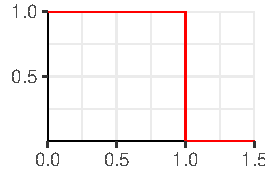
\includegraphics[scale=.4]{./img_ventanas/ventana_bartlett.pdf}\\
\rowcolor{gris}
Fejer &
$\displaystyle 
1-\abso{u}
$
& 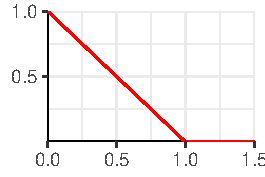
\includegraphics[scale=.4]{./img_ventanas/ventana_fejer.pdf} \\
Daniell &
$\displaystyle 
\frac{\SEN{\pi u}}{\pi u}
$
& 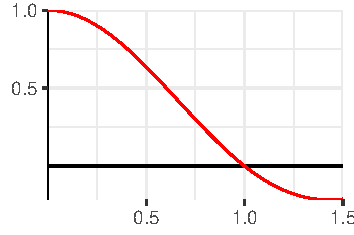
\includegraphics[scale=.4]{./img_ventanas/ventana_daniell.pdf} \\
\rowcolor{gris}
Bartlett-Priestley &
$\displaystyle 
\frac{3}{(\pi u)^{2}} \left[ \frac{\SEN{\pi u}}{\pi u} - \COS{\pi u} \right]
$
& 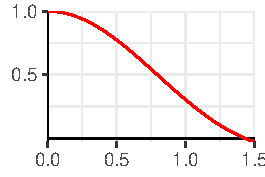
\includegraphics[scale=.4]{./img_ventanas/ventana_bartlet_priestley.pdf} \\
Cosenoidal &
$\displaystyle 
\COS{\pi u}
$
& 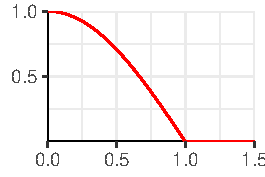
\includegraphics[scale=.4]{./img_ventanas/ventana_cosenoidal.pdf} \\
%\bottomrulec
\bottomrule
\end{tabular*}
\label{ventanas}
\end{SidewaysTable}

\begin{SidewaysTable}
\caption{Ejemplos de funciones ventana (función de transferencia)}
\centering
\begin{tabular}{lll}
\toprule
Nombre & $K(\theta)$ & Bosquejo \\
\midrule
Bartlett &
$\displaystyle 
\frac{1}{\pi} \frac{\SEN{\theta}}{\theta}
$
& 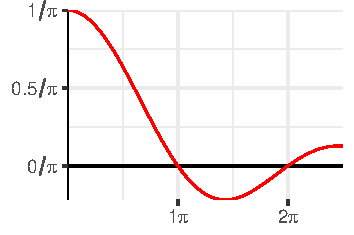
\includegraphics[scale=.4]{./img_ventanas/ventana_2_bartlett.pdf} \\
\rowcolor{gris}
Fejer &
$\displaystyle 
\frac{1}{2\pi} \left[ \frac{\SEN{\nicefrac{\theta}{2}}}{\nicefrac{\theta}{2}} \right]^{2}
$
& 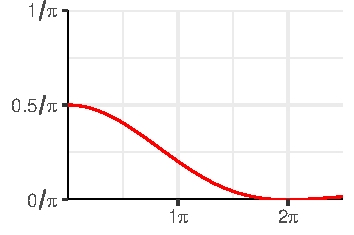
\includegraphics[scale=.4]{./img_ventanas/ventana_2_fejer.pdf} \\
Daniell &
$
\displaystyle 
\nicefrac{1}{2\pi} \text{, si } \abso{\theta}\leq \pi
$
& 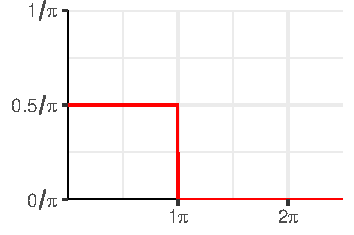
\includegraphics[scale=.4]{./img_ventanas/ventana_2_daniell.pdf} \\
\rowcolor{gris}
Bartlett-Priestley &
$\displaystyle 
\frac{3}{4 \pi} \left[ 1 - \left( \nicefrac{\theta}{\pi} \right) \right]
\text{, si } \abso{\theta}\leq \pi
$
& 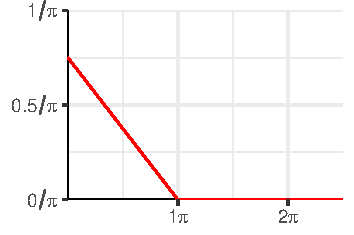
\includegraphics[scale=.4]{./img_ventanas/ventana_2_bartlet_priestley.pdf} \\
Cosenoidal &
$\displaystyle 
d
$
& 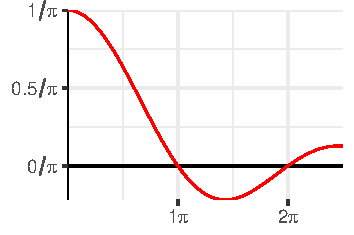
\includegraphics[scale=.4]{./img_ventanas/ventana_2_bartlett.pdf} \\
\bottomrule
\end{tabular}
\end{SidewaysTable}

%%%%%%%%%%%%%%%%%%%%%%%%%%%%%%%%%%%%%%%%%%%%%%%%%%%%%%%%%%%%%%%%%%%%%%%%%%%%%%%%%%%%%%%%%%%%%%%%%%%
%%%%%%%%%%%%%%%%%%%%%%%%%%%%%%%%%%%%%%%%%%%%%%%%%%%%%%%%%%%%%%%%%%%%%%%%%%%%%%%%%%%%%%%%%%%%%%%%%%%
%%%%%%%%%%%%%%%%%%%%%%%%%%%%%%%%%%%%%%%%%%%%%%%%%%%%%%%%%%%%%%%%%%%%%%%%%%%%%%%%%%%%%%%%%%%%%%%%%%%